\documentclass[11pt,a4paper]{article}

% =========================================================================
% PAKET-PAKET UTAMA
% =========================================================================
\usepackage[utf8]{inputenc}
\usepackage[T1]{fontenc}
\usepackage{lmodern}
\usepackage[indonesian]{babel}
\usepackage{amsmath,amssymb,amsfonts,amsthm}
\usepackage{bm}              % Notasi tebal untuk vektor & matriks
\usepackage{geometry}
\geometry{top=2.5cm, bottom=2.5cm, left=2.5cm, right=2.5cm}
\usepackage{graphicx}
\usepackage{booktabs}        % Tabel profesional
\usepackage{tabularx}
\usepackage{microtype}
\usepackage{tikz}            % Diagram skematis
\usetikzlibrary{matrix,decorations.pathreplacing,calc,positioning}
\usepackage{xcolor}
\usepackage{mdframed}        % Kotak highlight untuk pengerjaan soal
\usepackage{caption}
\usepackage{subcaption}
\usepackage{hyperref}
\hypersetup{
    colorlinks=true,
    linkcolor=blue!70!black,
    citecolor=blue!70!black,
    urlcolor=blue!70!black,
    pdfencoding=auto,
    psdextra
}
\pdfstringdefDisableCommands{%
  \def\boldsymbol#1{#1}%
  \def\bm#1{#1}%
  \def\mathbf#1{#1}%
}

% Pengaturan penomoran dan teorema
\newtheorem{definisi}{Definisi}[section]
\newtheorem{teorema}{Teorema}[section]
\newtheorem{catatan}{Catatan}[section]

% Path direktori gambar
\graphicspath{{figures/}}

% =========================================================================
% INFORMASI DOKUMEN
% =========================================================================
\title{
    \vspace{-1.0cm}
    \textbf{\Large DOKUMEN KREDIT BIMBINGAN TUGAS AKHIR \#2} \\[0.3em]
    \textbf{\large Fondasi Matematis, Penurunan Lengkap, Analisis Dimensi,}\\
    \textbf{\large dan Contoh Perhitungan Manual \textit{Gaussian Process Regression}}
}
\author{
    \textbf{Penulis / Mahasiswa}: Mahasiswa Tugas Akhir \\
    \textbf{Fokus Riset}: \textit{Image Segmentation with Deep Gaussian Process} \\
    \textbf{Target Pertemuan}: Bimbingan Rutin ke-2 (Rabu, 16 September 2026)
}
\date{\today}

\begin{document}

\maketitle
\vspace{-0.5cm}
\begin{abstract}
Dokumen kredit ini disusun sebagai pertanggungjawaban akademis berkala sekaligus tindak lanjut langsung dari evaluasi bimbingan perdana (9 September 2026). Dosen pembimbing menekankan urgensi penguasaan fondasi teoretis, definisi formal, serta ketelitian matematis dari \textit{Gaussian Process} (GP) sebelum melangkah ke arsitektur tingkat lanjut (\textit{Deep Gaussian Process}). Dokumen ini menyajikan pembuktian matematis yang komprehensif mengenai \textit{Gaussian Process Regression} (GPR). Setiap entitas simbolik didefinisikan secara eksplisit sifat aljabarnya (skalar, vektor, matriks) beserta dimensi ruangnya ($\mathbb{R}^D, \mathbb{R}^N$). Lebih lanjut, dokumen ini menyajikan contoh perhitungan manual langkah demi langkah (\textit{worked homework example}) menggunakan dekomposisi Cholesky stabil untuk $N = 3$ titik training data dan $N_* = 2$ titik test data lengkap dengan grafik hasil numerik dan interpretasi fisis mengenai \textit{epistemic uncertainty}.
\end{abstract}

\hrule
\vspace{0.3cm}
\tableofcontents
\vspace{0.4cm}
\hrule

\newpage

% =========================================================================
% BAGIAN 1: KONVENSI NOTASI & DIMENSI
% =========================================================================
\section{Konvensi Tipografi dan Dimensi Matematis}
\label{sec:notasi}

Untuk memastikan ketelitian aljabar linier dan menghindari kerancuan notasi, dokumen ini menerapkan konvensi tipografi dan dimensi standar sebagaimana dirangkum pada Tabel~\ref{tab:notasi}.

\begin{table}[h!]
\centering
\small
\caption{Konvensi Notasi dan Dimensi Ruang Aljabar Linier.}
\label{tab:notasi}
\begin{tabularx}{\textwidth}{l c l X}
\toprule
\textbf{Kategori Entitas} & \textbf{Simbol Contoh} & \textbf{Ruang Dimensi} & \textbf{Deskripsi / Peran Matematis} \\
\midrule
Jumlah Training Samples & $N$ & $\mathbb{N}$ & Skalar bulat: Banyaknya observasi dalam training dataset. \\
Jumlah Test Points & $N_*$ & $\mathbb{N}$ & Skalar bulat: Banyaknya lokasi target prediksi/inferensi. \\
Dimensi Input Fitur & $D$ & $\mathbb{N}$ & Skalar bulat: Banyaknya koordinat/fitur pada domain input. \\
\midrule
Titik Input Observasi & $\mathbf{x}_i$ & $\mathbb{R}^{D \times 1}$ & Vektor kolom: Koordinat spasial atau fitur sampel ke-$i$. \\
Matriks Desain Training & $X$ & $\mathbb{R}^{N \times D}$ & Matriks training input bertumpuk, $X = [\mathbf{x}_1, \dots, \mathbf{x}_N]^T$. \\
Matriks Desain Test & $X_*$ & $\mathbb{R}^{N_* \times D}$ & Matriks input test point, $X_* = [\mathbf{x}_{*1}, \dots, \mathbf{x}_{*N_*}]^T$. \\
\midrule
Target Observasi & $y_i$ & $\mathbb{R}$ & Skalar riil: Nilai target tercemar noise pada titik $\mathbf{x}_i$. \\
Vektor Target Training & $\mathbf{y}$ & $\mathbb{R}^{N \times 1}$ & Vektor kolom observed training data, $\mathbf{y} = [y_1, \dots, y_N]^T$. \\
Fungsi Laten Training & $\mathbf{f}$ & $\mathbb{R}^{N \times 1}$ & Vektor nilai fungsi murni tanpa noise, $\mathbf{f} = [f(\mathbf{x}_1), \dots, f(\mathbf{x}_N)]^T$. \\
Vektor Derau Observasi & $\boldsymbol{\epsilon}$ & $\mathbb{R}^{N \times 1}$ & Vektor residu noise Gaussian, $\boldsymbol{\epsilon} \sim \mathcal{N}(\mathbf{0}, \sigma_n^2 I_N)$. \\
Fungsi Laten Test & $\mathbf{f}_*$ & $\mathbb{R}^{N_* \times 1}$ & Vektor variabel acak nilai fungsi laten yang diprediksi. \\
\midrule
Kovariansi Antar Training Data & $K(X, X)$ & $\mathbb{R}^{N \times N}$ & Matriks Gram simetris positif semi-definit dari fungsi kernel. \\
Kovariansi Total Training Data & $K_y$ & $\mathbb{R}^{N \times N}$ & Matriks kovariansi ber-noise, $K_y = K(X,X) + \sigma_n^2 I_N$. \\
Kovariansi Training-Test & $K(X, X_*)$ & $\mathbb{R}^{N \times N_*}$ & Matriks kovariansi silang antara training points dan test point. \\
Kovariansi Test-Training & $K(X_*, X)$ & $\mathbb{R}^{N_* \times N}$ & Transpose dari matriks silang, $K(X_*, X) = K(X, X_*)^T$. \\
Kovariansi Antar Test Points & $K(X_*, X_*)$ & $\mathbb{R}^{N_* \times N_*}$ & Matriks kovariansi internal antar sesama test point. \\
\midrule
Faktor Cholesky & $L$ & $\mathbb{R}^{N \times N}$ & Matriks segitiga bawah riil (\textit{lower triangular}), $K_y = L L^T$. \\
Vektor Bobot Prediktif & $\boldsymbol{\alpha}$ & $\mathbb{R}^{N \times 1}$ & Vektor solusi sistem linier, $\boldsymbol{\alpha} = K_y^{-1} \mathbf{y} = L^{-T} L^{-1} \mathbf{y}$. \\
Vektor Mean Prediktif & $\bar{\mathbf{f}}_*$ & $\mathbb{R}^{N_* \times 1}$ & Ekspektasi nilai fungsi posterior pada test point $X_*$. \\
Kovariansi Prediktif & $\operatorname{cov}(\mathbf{f}_*)$ & $\mathbb{R}^{N_* \times N_*}$ & Matriks ketidakpastian posterior pada test point $X_*$. \\
Variansi Individual Test Point & $\mathbb{V}[f_{*j}]$ & $\mathbb{R}^+$ & Skalar variansi marjinal test point ke-$j$, yaitu $[\operatorname{cov}(\mathbf{f}_*)]_{jj}$. \\
\bottomrule
\end{tabularx}
\end{table}

% =========================================================================
% BAGIAN 2: PENDAHULUAN & FILOSOFI BAYESIAN
% =========================================================================
\section{Pendahuluan \& Pandangan Ruang-Fungsi (\textit{Function-Space View})}
\label{sec:filosofi}

Dalam pembelajaran mesin konvensional berparadigma parametrik, regresi linear memodelkan relasi fungsional melalui kombinasi linear berbobot:
\begin{equation}
y = \mathbf{w}^T \boldsymbol{\phi}(\mathbf{x}) + \epsilon, \quad \mathbf{w} \in \mathbb{R}^{H \times 1}, \; \boldsymbol{\phi}(\mathbf{x}) \in \mathbb{R}^{H \times 1}, \; \epsilon \sim \mathcal{N}(0, \sigma_n^2)
\end{equation}
di mana inferensi Bayesian dilakukan dengan menempatkan distribusi prior atas ruang parameter bobot: $\mathbf{w} \sim \mathcal{N}(\mathbf{0}, \Sigma_p)$.

Sebaliknya, \textit{Gaussian Process} (GP) mengadopsi sudut pandang \textbf{ruang-fungsi} (\textit{function-space view}). GP memotong perantara parameter $\mathbf{w}$ dan menempatkan prior probabilitas secara langsung di atas ruang fungsi tak berhingga $f(\mathbf{x})$.

\begin{definisi}[\textbf{Gaussian Process}]
Suatu \textbf{Gaussian Process} adalah koleksi variabel acak $\{f(\mathbf{x}) \mid \mathbf{x} \in \mathcal{X}\}$ di mana setiap subset berhingga dari indeks $\{\mathbf{x}_1, \dots, \mathbf{x}_N\}$ menghasilkan distribusi bersama (\textit{joint distribution}) multivariat Gaussian.
\end{definisi}

Secara matematis, Gaussian Process dispesifikasikan secara utuh oleh sebuah \textbf{fungsi mean} $m(\mathbf{x}) \in \mathbb{R}$ dan sebuah \textbf{fungsi kovariansi / kernel} $k(\mathbf{x}, \mathbf{x}') \in \mathbb{R}$:
\begin{align}
m(\mathbf{x}) &= \mathbb{E}[f(\mathbf{x})], \\
k(\mathbf{x}, \mathbf{x}') &= \mathbb{E}\big[ (f(\mathbf{x}) - m(\mathbf{x}))(f(\mathbf{x}') - m(\mathbf{x}')) \big]
\end{align}
sehingga proses stokastik ini dinotasikan sebagai:
\begin{equation}
f(\mathbf{x}) \sim \mathcal{GP}\big(m(\mathbf{x}), k(\mathbf{x}, \mathbf{x}')\big)
\end{equation}

\begin{catatan}[\textbf{Asumsi Mean Nol Tanpa Kehilangan Generalitas}]
Dalam praktik riset machine learning dan literatur standar Rasmussen \& Williams (2006), fungsi mean sering diasumsikan bernilai nol di mana-mana, yaitu $m(\mathbf{x}) \equiv 0$. Asumsi ini tidak membatasi fleksibilitas model karena nilai rata-rata data observasi $\mathbf{y}$ dapat dinormalisasi terlebih dahulu, dan nilai ekspektasi posterior akan sepenuhnya dikendalikan oleh data observasi melalui fungsi kernel.
\end{catatan}

\begin{figure}[h!]
\centering
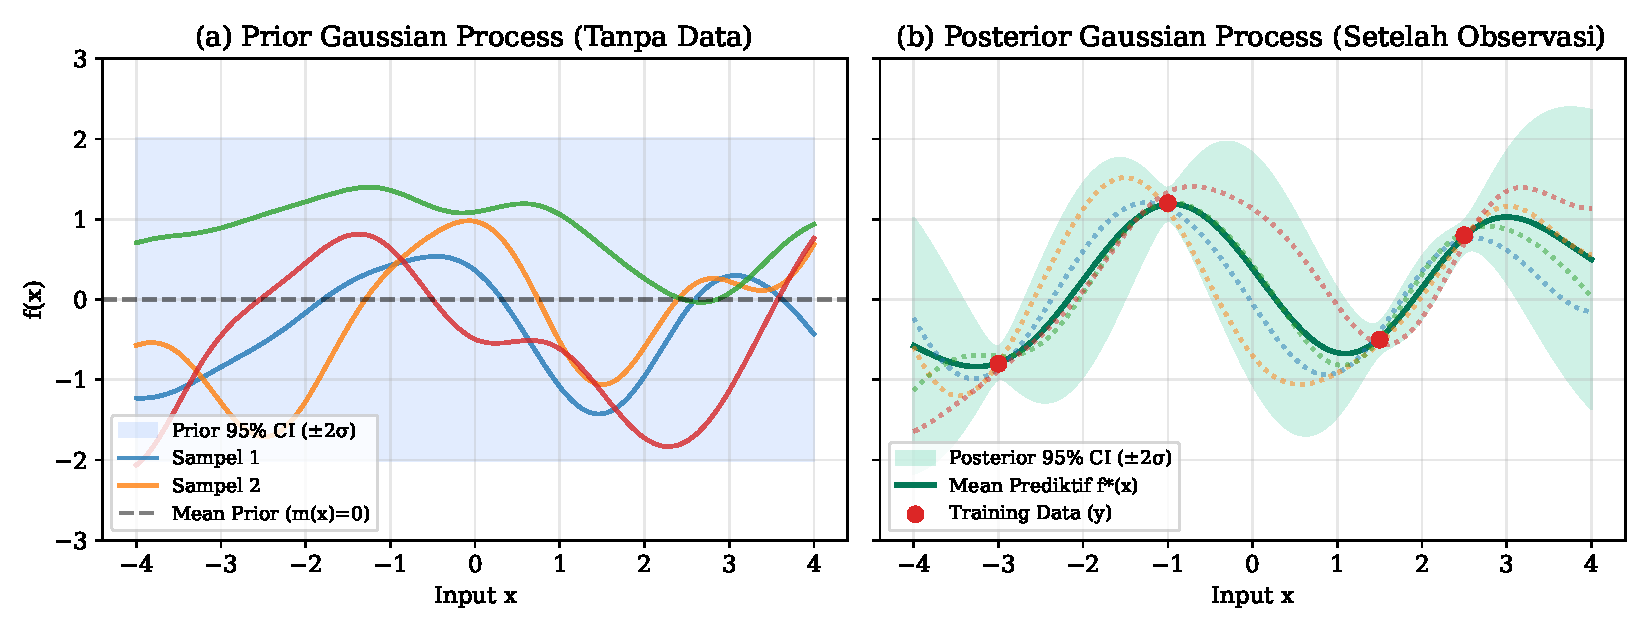
\includegraphics[width=0.95\textwidth]{fig1_prior_posterior.pdf}
\caption{Visualisasi Konseptual Gaussian Process: (a) Sampel-sampel fungsi prior yang ditarik dari $\mathcal{GP}(0, k(\mathbf{x},\mathbf{x}'))$ dengan pita ketidakpastian konstan $95\%$, dan (b) Sampel-sampel fungsi posterior setelah mengamati empat titik training data, memperlihatkan penyempitan pita ketidakpastian di sekitar titik data.}
\label{fig:prior_posterior}
\end{figure}

% =========================================================================
% BAGIAN 3: KOVARIANSI & FUNGSI KERNEL
% =========================================================================
\section{Kovariansi, Karakteristik Fungsi Kernel, dan Hyperparameter}
\label{sec:kernel}

Fungsi kovariansi $k(\mathbf{x}, \mathbf{x}')$ mendefinisikan korelasi spasial antara dua titik masukan: jika input $\mathbf{x}$ dan $\mathbf{x}'$ berdekatan dalam ruang input, maka nilai fungsi $f(\mathbf{x})$ dan $f(\mathbf{x}')$ harus berkorelasi tinggi (nilainya mirip).

\subsection{Syarat Kelayakan Kernel (Positive Semi-Definite)}
Agar matriks kovariansi $K \in \mathbb{R}^{N \times N}$ merepresentasikan distribusi Gaussian multivariat yang valid, matriks $K$ wajib bersifat \textbf{simetris dan positif semi-definit} (PSD). Artinya, untuk setiap himpunan titik $\{ \mathbf{x}_i \}_{i=1}^N$ dan vektor bobot sembarang $\mathbf{v} \in \mathbb{R}^{N \times 1} \setminus \{\mathbf{0}\}$, berlaku:
\begin{equation}
\mathbf{v}^T K \mathbf{v} = \sum_{i=1}^N \sum_{j=1}^N v_i v_j k(\mathbf{x}_i, \mathbf{x}_j) \ge 0
\end{equation}
Kondisi ini dijamin secara teoretis oleh \textit{Teorema Mercer} dan \textit{Teorema Bochner}.

\subsection{Kernel Squared Exponential (RBF / Gaussian)}
Kernel yang paling luas digunakan adalah \textit{Squared Exponential} (SE):
\begin{equation}
k_{\mathrm{SE}}(\mathbf{x}, \mathbf{x}') = \sigma_f^2 \exp\left( -\frac{\|\mathbf{x} - \mathbf{x}'\|^2}{2 l^2} \right) = \sigma_f^2 \exp\left( -\frac{(\mathbf{x} - \mathbf{x}')^T(\mathbf{x} - \mathbf{x}')}{2 l^2} \right)
\end{equation}
di mana:
\begin{itemize}
    \item $\sigma_f^2 \in \mathbb{R}^+$ (skalar): Amplitudo variansi sinyal vertikal, mengatur deviasi tipikal nilai fungsi menjauhi mean.
    \item $l \in \mathbb{R}^+$ (skalar): \textit{Characteristic lengthscale}, mengatur seberapa cepat korelasi meluruh terhadap jarak horizontal di ruang input.
\end{itemize}

\begin{catatan}[\textbf{Keteraturan Fungsi RBF}]
Kernel RBF bersifat \textit{infinitely mean-square differentiable} ($C^\infty$). Artinya, sampel fungsi dari kernel RBF memiliki turunan hingga orde tak hingga, menghasilkan kurva yang luar biasa mulus (\textit{infinitely smooth}).
\end{catatan}

\subsection{Keluarga Kernel Matérn}
Dalam aplikasi fisik, geofisika, maupun pemrosesan citra, asumsi kemulusan tak hingga dari RBF sering kali tidak realistis karena pola data riil memiliki perubahan lokal yang tajam. Keluarga kernel Matérn mengatasi masalah ini:
\begin{equation}
k_{\mathrm{Mat\acute{e}rn}}(r) = \sigma_f^2 \frac{2^{1-\nu}}{\Gamma(\nu)} \left( \frac{\sqrt{2\nu} r}{l} \right)^\nu K_\nu\left( \frac{\sqrt{2\nu} r}{l} \right)
\end{equation}
di mana $r = \|\mathbf{x} - \mathbf{x}'\| \in \mathbb{R}^+$ adalah jarak Euclidean, $\Gamma(\cdot)$ adalah fungsi Gamma, dan $K_\nu(\cdot)$ adalah fungsi Bessel termodifikasi jenis ketiga orde $\nu$. Dua nilai $\nu$ yang paling lazim dalam literatur adalah:
\begin{itemize}
    \item \textbf{Matérn $\nu = 3/2$} (dapat diturunkan 1 kali / $C^1$ differentiable):
    \begin{equation}
    k_{\nu=3/2}(r) = \sigma_f^2 \left( 1 + \frac{\sqrt{3}r}{l} \right) \exp\left( -\frac{\sqrt{3}r}{l} \right)
    \end{equation}
    \item \textbf{Matérn $\nu = 5/2$} (dapat diturunkan 2 kali / $C^2$ differentiable):
    \begin{equation}
    k_{\nu=5/2}(r) = \sigma_f^2 \left( 1 + \frac{\sqrt{5}r}{l} + \frac{5r^2}{3l^2} \right) \exp\left( -\frac{\sqrt{5}r}{l} \right)
    \end{equation}
\end{itemize}

\begin{figure}[h!]
\centering
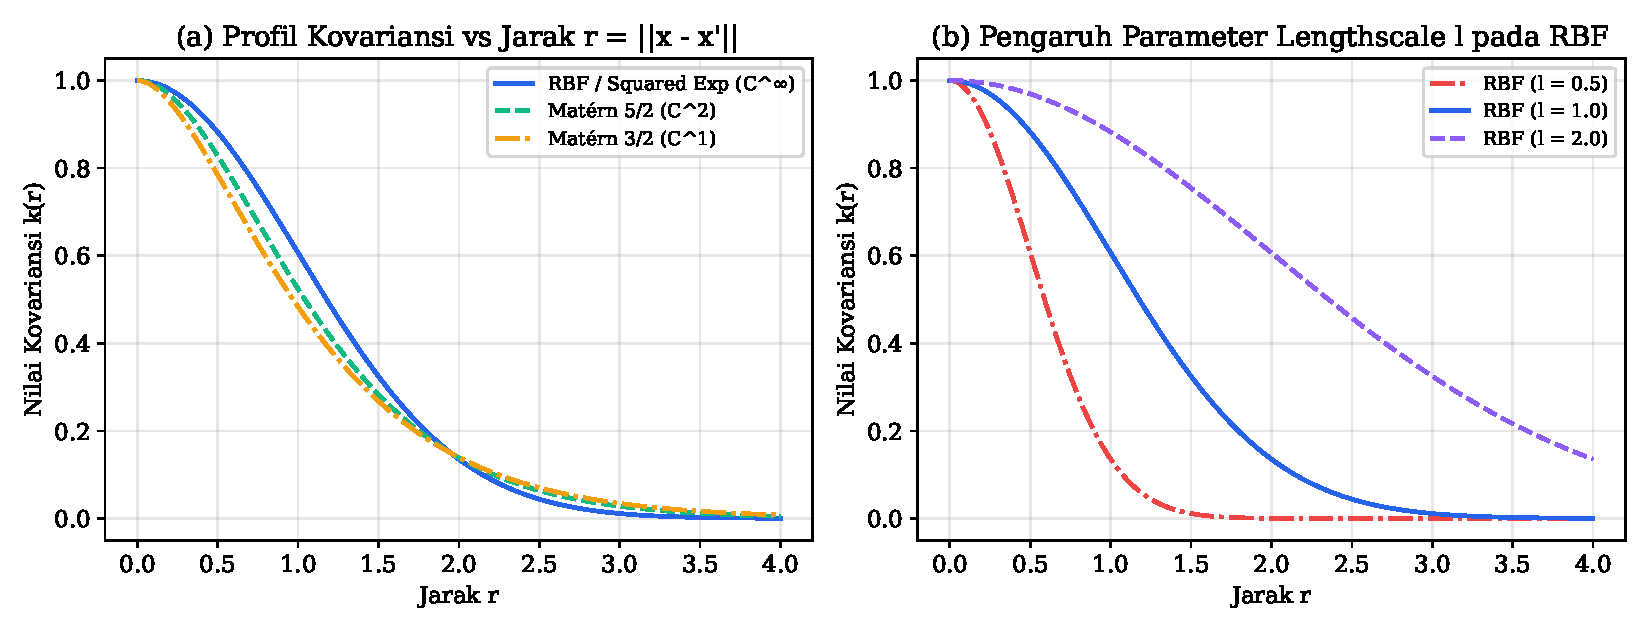
\includegraphics[width=0.95\textwidth]{fig2_kernel_profiles.pdf}
\caption{Perbandingan Sifat Kernel: (a) Peluruhan nilai kovariansi $k(r)$ terhadap jarak spasial $r$ antara RBF, Matérn 5/2, dan Matérn 3/2, dan (b) Pengaruh parameter \textit{lengthscale} $l$ dalam mengontrol jangkauan pengaruh spasial.}
\label{fig:kernel_profiles}
\end{figure}

% =========================================================================
% BAGIAN 4: MODEL REGRESI BER-NOISE
% =========================================================================
\section{Formulasi Model Regresi dengan Noise Observasi}
\label{sec:model_regresi}

Dalam skenario observasi riil, data target yang kita amati tercemar oleh ketidakpastian sensorik atau derau pengukuran (\textit{aleatoric noise}). Model regresi didefinisikan sebagai:
\begin{equation}
y_i = f(\mathbf{x}_i) + \epsilon_i, \quad i = 1, \dots, N
\end{equation}
di mana residu derau diasumsikan saling bebas dan berdistribusi identik (\textit{i.i.d.}) Gaussian:
\begin{equation}
\epsilon_i \sim \mathcal{N}(0, \sigma_n^2) \implies \boldsymbol{\epsilon} = [\epsilon_1, \dots, \epsilon_N]^T \sim \mathcal{N}(\mathbf{0}_{N \times 1}, \sigma_n^2 I_N)
\end{equation}
di mana $\sigma_n^2 \in \mathbb{R}^+$ adalah variansi noise (skalar) dan $I_N \in \mathbb{R}^{N \times N}$ adalah matriks identitas.

Kovariansi antara dua observasi sembarang $y_p$ dan $y_q$ dapat diturunkan langsung dari sifat ekspektasi linearitas:
\begin{align}
\operatorname{cov}(y_p, y_q) &= \mathbb{E}[(y_p - 0)(y_q - 0)] \nonumber \\
&= \mathbb{E}\big[ (f(\mathbf{x}_p) + \epsilon_p)(f(\mathbf{x}_q) + \epsilon_q) \big] \nonumber \\
&= \mathbb{E}[f(\mathbf{x}_p)f(\mathbf{x}_q)] + \mathbb{E}[f(\mathbf{x}_p)\epsilon_q] + \mathbb{E}[\epsilon_p f(\mathbf{x}_q)] + \mathbb{E}[\epsilon_p \epsilon_q] \nonumber \\
&= k(\mathbf{x}_p, \mathbf{x}_q) + 0 + 0 + \sigma_n^2 \delta_{pq}
\end{align}
di mana $\delta_{pq}$ adalah fungsi delta Kronecker ($\delta_{pq} = 1$ jika $p=q$, dan $0$ jika $p \neq q$).

Dalam notasi matriks penuh, matriks kovariansi observed training data $K_y \in \mathbb{R}^{N \times N}$ dirumuskan sebagai:
\begin{equation}
\label{eq:Ky}
K_y = K(X, X) + \sigma_n^2 I_N \in \mathbb{R}^{N \times N}
\end{equation}
dengan elemen matriks $[K(X, X)]_{ij} = k(\mathbf{x}_i, \mathbf{x}_j)$.

% =========================================================================
% BAGIAN 5: PENURUNAN ANALITIK POSTERIOR
% =========================================================================
\section{Penurunan Analitik Distribusi Bersyarat Posterior (\textit{Conditioning})}
\label{sec:posterior_derivation}

Misalkan diberikan himpunan $N_*$ test input points yang disusun dalam matriks $X_* \in \mathbb{R}^{N_* \times D}$. Tujuan inferensi Bayesian adalah memperoleh distribusi probabilitas bersyarat dari nilai fungsi laten test $\mathbf{f}_* = [f(\mathbf{x}_{*1}), \dots, f(\mathbf{x}_{*N_*})]^T \in \mathbb{R}^{N_* \times 1}$ dengan syarat training data yang diobservasi $(X, \mathbf{y})$, yaitu:
\begin{equation}
p(\mathbf{f}_* \mid X, \mathbf{y}, X_*)
\end{equation}

\subsection{Distribusi Gabungan Prior (Joint Gaussian Prior)}
Berdasarkan definisi dasar Gaussian Process, kumpulan observasi $\mathbf{y} \in \mathbb{R}^{N \times 1}$ dan fungsi laten test $\mathbf{f}_* \in \mathbb{R}^{N_* \times 1}$ secara bersama-sama membentuk distribusi Gaussian multivariat berdimensi $(N + N_*)$:
\begin{equation}
\label{eq:joint_prior}
\begin{bmatrix} \mathbf{y} \\ \mathbf{f}_* \end{bmatrix} \sim \mathcal{N}\left(
\begin{bmatrix} \mathbf{0}_{N \times 1} \\ \mathbf{0}_{N_* \times 1} \end{bmatrix},
\begin{bmatrix}
K_y & K(X, X_*) \\
K(X_*, X) & K(X_*, X_*)
\end{bmatrix}
\right)
\end{equation}
Struktur partisi blok matriks kovariansi pada Persamaan~\eqref{eq:joint_prior} diilustrasikan secara diagramatis pada Gambar~\ref{fig:tikz_joint_matrix}.

\begin{figure}[h!]
\centering
\begin{tikzpicture}[scale=0.95]
    % Matriks Blok Luar
    \draw[thick, fill=blue!5] (0,0) rectangle (7,7);
    \draw[dashed, line width=1pt, red!70!black] (0,2.5) -- (7,2.5);
    \draw[dashed, line width=1pt, red!70!black] (4.5,0) -- (4.5,7);

    % Label Blok K_y
    \node at (2.25, 4.75) [align=center] {
        \textbf{\large $K_y = K(X,X) + \sigma_n^2 I_N$} \\
        \small Dimensi: $N \times N$ \\
        \footnotesize (Kovariansi Training Data Ber-Noise)
    };

    % Label Blok K(X, X_*)
    \node at (5.75, 4.75) [align=center] {
        \textbf{\large $K(X, X_*)$} \\
        \small Dimensi: $N \times N_*$ \\
        \footnotesize (Kovariansi Silang)
    };

    % Label Blok K(X_*, X)
    \node at (2.25, 1.25) [align=center] {
        \textbf{\large $K(X_*, X)$} \\
        \small Dimensi: $N_* \times N$ \\
        \footnotesize ($= K(X, X_*)^T$)
    };

    % Label Blok K(X_*, X_*)
    \node at (5.75, 1.25) [align=center] {
        \textbf{\large $K(X_*, X_*)$} \\
        \small Dimensi: $N_* \times N_*$ \\
        \footnotesize (Prior Titik Test)
    };

    % Anotasi Kurung Kurawal
    \draw [decorate,decoration={brace,amplitude=8pt,mirror,raise=4pt},thick]
    (0,0) -- (4.5,0) node [midway,yshift=-20pt] {\small Training Data $N$};
    \draw [decorate,decoration={brace,amplitude=8pt,mirror,raise=4pt},thick]
    (4.5,0) -- (7,0) node [midway,yshift=-20pt] {\small Test Data $N_*$};

    \draw [decorate,decoration={brace,amplitude=8pt,raise=4pt},thick]
    (0,2.5) -- (0,7) node [midway,xshift=-25pt,rotate=90] {\small Training Data $N$};
    \draw [decorate,decoration={brace,amplitude=8pt,raise=4pt},thick]
    (0,0) -- (0,2.5) node [midway,xshift=-25pt,rotate=90] {\small Test Data $N_*$};
\end{tikzpicture}
\caption{Diagram Partisi Blok Matriks Kovariansi Bersama (\textit{Joint Covariance Matrix}). Matriks berukuran $(N + N_*) \times (N + N_*)$ terbagi menjadi 4 submatriks yang mencerminkan interaksi antara training data dan test data.}
\label{fig:tikz_joint_matrix}
\end{figure}

\subsection{Teorema Partisi Gaussian Bersyarat (Schur Complement)}
\begin{teorema}[\textbf{Conditioning pada Multivariat Normal}]
\label{thm:conditioning}
Misalkan sebuah vektor acak terpartisi $\mathbf{z} = [\mathbf{z}_A^T, \mathbf{z}_B^T]^T$ berdistribusi Gaussian gabungan:
\begin{equation}
\begin{bmatrix} \mathbf{z}_A \\ \mathbf{z}_B \end{bmatrix} \sim \mathcal{N}\left(
\begin{bmatrix} \boldsymbol{\mu}_A \\ \boldsymbol{\mu}_B \end{bmatrix},
\begin{bmatrix} \Sigma_{AA} & \Sigma_{AB} \\ \Sigma_{BA} & \Sigma_{BB} \end{bmatrix}
\right)
\end{equation}
di mana $\Sigma_{BA} = \Sigma_{AB}^T$. Maka distribusi bersyarat dari $\mathbf{z}_B$ dengan syarat $\mathbf{z}_A$ juga berdistribusi Gaussian secara eksak:
\begin{equation}
\mathbf{z}_B \mid \mathbf{z}_A \sim \mathcal{N}(\boldsymbol{\mu}_{B|A}, \Sigma_{B|A})
\end{equation}
dengan mean dan kovariansi analitik:
\begin{align}
\boldsymbol{\mu}_{B|A} &= \boldsymbol{\mu}_B + \Sigma_{BA} \Sigma_{AA}^{-1} (\mathbf{z}_A - \boldsymbol{\mu}_A) \\
\Sigma_{B|A} &= \Sigma_{BB} - \Sigma_{BA} \Sigma_{AA}^{-1} \Sigma_{AB}
\end{align}
\end{teorema}

\begin{proof}[\textbf{Sketsa Penurunan Matematis}]
Matriks kovariansi bersama $\Sigma$ dapat difaktorisasi ke dalam bentuk blok diagonal melalui eliminasi blok Gauss (\textit{Schur Complement}). Fungsi kepekatan probabilitas bersama adalah $p(\mathbf{z}_A, \mathbf{z}_B) \propto \exp\left(-\frac{1}{2} (\mathbf{z} - \boldsymbol{\mu})^T \Sigma^{-1} (\mathbf{z} - \boldsymbol{\mu})\right)$. Dengan memanfaatkan rumus inversi blok matriks Frobenius/Banachiewicz:
\begin{equation}
\Sigma^{-1} = \begin{bmatrix} I & -\Sigma_{AA}^{-1} \Sigma_{AB} \\ 0 & I \end{bmatrix}
\begin{bmatrix} \Sigma_{AA}^{-1} & 0 \\ 0 & (\Sigma_{BB} - \Sigma_{BA}\Sigma_{AA}^{-1}\Sigma_{AB})^{-1} \end{bmatrix}
\begin{bmatrix} I & 0 \\ -\Sigma_{BA}\Sigma_{AA}^{-1} & I \end{bmatrix}
\end{equation}
Bentuk kuadratik pada eksponen terfaktorisasi sempurna menjadi jumlahan kuadrat terhadap $\mathbf{z}_A$ dan bentuk kuadratik terhadap $(\mathbf{z}_B - \boldsymbol{\mu}_{B|A})$. Karena $p(\mathbf{z}_B \mid \mathbf{z}_A) = \frac{p(\mathbf{z}_A, \mathbf{z}_B)}{p(\mathbf{z}_A)}$, faktor yang hanya bergantung pada $\mathbf{z}_A$ saling mengeliminasi pada pembilang dan penyebut, meninggalkan distribusi normal univariat/multivariat dengan mean $\boldsymbol{\mu}_{B|A}$ dan kovariansi $\Sigma_{B|A}$.
\end{proof}

\subsection{Formulasi Eksplisit Posterior GPR}
Dengan mensubstitusikan korespondensi variabel dari model kita:
\begin{equation}
\mathbf{z}_A \leftarrow \mathbf{y}, \quad \mathbf{z}_B \leftarrow \mathbf{f}_*, \quad \boldsymbol{\mu}_A \leftarrow \mathbf{0}_{N \times 1}, \quad \boldsymbol{\mu}_B \leftarrow \mathbf{0}_{N_* \times 1}
\end{equation}
\begin{equation}
\Sigma_{AA} \leftarrow K_y = K(X,X) + \sigma_n^2 I_N, \quad \Sigma_{AB} \leftarrow K(X, X_*), \quad \Sigma_{BA} \leftarrow K(X_*, X), \quad \Sigma_{BB} \leftarrow K(X_*, X_*)
\end{equation}
maka kita peroleh \textbf{Teorema Fundamental Gaussian Process Regression}:
\begin{mdframed}[linewidth=1.2pt, linecolor=blue!70!black, backgroundcolor=blue!2]
\textbf{Distribusi Posterior Gaussian Process Regression}:
\begin{equation}
\mathbf{f}_* \mid X, \mathbf{y}, X_* \sim \mathcal{N}\big( \bar{\mathbf{f}}_*, \operatorname{cov}(\mathbf{f}_*) \big)
\end{equation}
\begin{align}
\label{eq:posterior_mean}
\bar{\mathbf{f}}_* &= K(X_*, X) \left[ K(X, X) + \sigma_n^2 I_N \right]^{-1} \mathbf{y} \in \mathbb{R}^{N_* \times 1} \\
\label{eq:posterior_cov}
\operatorname{cov}(\mathbf{f}_*) &= K(X_*, X_*) - K(X_*, X) \left[ K(X, X) + \sigma_n^2 I_N \right]^{-1} K(X, X_*) \in \mathbb{R}^{N_* \times N_*}
\end{align}
\end{mdframed}

Untuk kasus test point tunggal $\mathbf{x}_* \in \mathbb{R}^{D \times 1}$ ($N_* = 1$), notasi vektor disederhanakan menjadi $\mathbf{k}_* = K(X, \mathbf{x}_*) \in \mathbb{R}^{N \times 1}$ dan skalar $k_{**} = k(\mathbf{x}_*, \mathbf{x}_*) \in \mathbb{R}$:
\begin{align}
\bar{f}_* &= \mathbf{k}_*^T K_y^{-1} \mathbf{y} \quad \in \mathbb{R} \quad \text{\footnotesize (Dimensi: $(1 \times N) \times (N \times N) \times (N \times 1) = 1 \times 1$)} \\
\mathbb{V}[f_*] &= k_{**} - \mathbf{k}_*^T K_y^{-1} \mathbf{k}_* \quad \in \mathbb{R}^+ \quad \text{\footnotesize (Dimensi: $1 - (1 \times N) \times (N \times N) \times (N \times 1) = 1 \times 1$)}
\end{align}

\subsection{Sifat-Sifat Fisis dan Probabilistik Posterior}
\begin{enumerate}
    \item \textbf{Representasi Dual}: Mean posterior dapat dinyatakan sebagai ekspansi fungsi kernel $\bar{f}_* = \sum_{i=1}^N \alpha_i k(\mathbf{x}_i, \mathbf{x}_*)$ di mana $\boldsymbol{\alpha} = K_y^{-1}\mathbf{y} \in \mathbb{R}^{N \times 1}$. Ini membuktikan teorema representasi dasar bahwa prediksi merupakan kombinasi linear fungsi basis yang berpusat pada training data.
    \item \textbf{Independensi Variansi dari Label Data}: Persamaan~\eqref{eq:posterior_cov} membuktikan bahwa kovariansi posterior $\operatorname{cov}(\mathbf{f}_*)$ \textbf{sama sekali tidak bergantung} pada nilai target $\mathbf{y}$. Ketidakpastian hanya dikendalikan oleh posisi spasial relatif input $X$ dan $X_*$.
    \item \textbf{Pemodelan Epistemic Uncertainty}: Di sekitar data observasi ($X_* \approx X$), suku pengurang mendekati nilai prior sehingga $\mathbb{V}[f_*] \to \sigma_n^2$ (ketidakpastian menyusut). Sebaliknya, pada daerah ekstrapolasi yang jauh dari training data, suku pengurang mendekati nol sehingga $\mathbb{V}[f_*] \to k_{**} = \sigma_f^2$ (model kembali ke status keraguan penuh sesuai prior).
\end{enumerate}

% =========================================================================
% BAGIAN 6: OPTIMASI MARGINAL LIKELIHOOD
% =========================================================================
\section{Optimasi Hyperparameter via Marginal Likelihood}
\label{sec:marginal_likelihood}

Kinerja model Gaussian Process bergantung pada pemilihan vektor hyperparameter kernel $\boldsymbol{\theta} = [\sigma_f^2, l, \sigma_n^2]^T \in \mathbb{R}^{P \times 1}$. Pendekatan Bayesian yang paling elegan dan objektif adalah memaksimumkan \textbf{Marginal Likelihood} (\textit{Evidence}).

\subsection{Integrasi Marjinal Analitik}
Marginal likelihood mengintegralkan keluar (\textit{marginalizes}) seluruh kemungkinan fungsi laten $\mathbf{f} \in \mathbb{R}^{N \times 1}$:
\begin{equation}
p(\mathbf{y} \mid X, \boldsymbol{\theta}) = \int_{\mathbb{R}^N} p(\mathbf{y} \mid \mathbf{f}) \, p(\mathbf{f} \mid X, \boldsymbol{\theta}) \, d\mathbf{f}
\end{equation}
Karena likelihood $p(\mathbf{y} \mid \mathbf{f}) = \mathcal{N}(\mathbf{f}, \sigma_n^2 I_N)$ dan prior $p(\mathbf{f} \mid X, \boldsymbol{\theta}) = \mathcal{N}(\mathbf{0}, K(X,X))$ keduanya merupakan distribusi normal, hasil konvolusi integral Gaussian menghasilkan distribusi normal tertutup secara analitik:
\begin{equation}
\mathbf{y} \mid X, \boldsymbol{\theta} \sim \mathcal{N}(\mathbf{0}_{N \times 1}, K_y)
\end{equation}
di mana $K_y = K(X,X) + \sigma_n^2 I_N$.

\subsection{Formulasi Log Marginal Likelihood (LML) dan Prinsip Occam's Razor}
Dengan mengambil nilai logaritma natural dari fungsi kepekatan probabilitas multivariat Gaussian di atas, kita peroleh fungsi objektif \textbf{Log Marginal Likelihood} (LML):
\begin{equation}
\label{eq:lml}
\log p(\mathbf{y} \mid X, \boldsymbol{\theta}) = \underbrace{-\frac{1}{2} \mathbf{y}^T K_y^{-1} \mathbf{y}}_{\text{Data-fit term}} \; \underbrace{-\frac{1}{2} \log |K_y|}_{\text{Complexity penalty}} \; \underbrace{-\frac{N}{2} \log(2\pi)}_{\text{Normalizing constant}}
\end{equation}

\begin{figure}[h!]
\centering
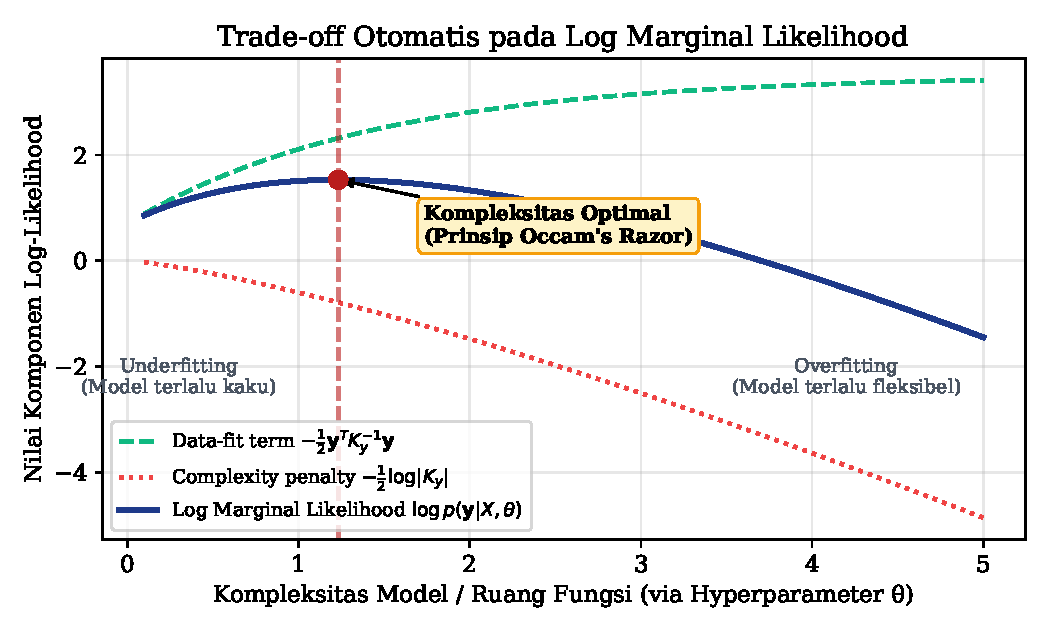
\includegraphics[width=0.7\textwidth]{fig4_occams_razor.pdf}
\caption{Visualisasi Prinsip Occam's Razor Otomatis pada Log Marginal Likelihood: Interaksi trade-off antara peningkatan kesesuaian data (\textit{data-fit}) dan penalti volume ruang fungsi (\textit{complexity penalty}) menghasilkan titik puncak optimum tunggal tanpa memerlukan validasi silang (\textit{cross-validation}).}
\label{fig:occams_razor}
\end{figure}

Dekonstruksi matematis Persamaan~\eqref{eq:lml} (sebagaimana divisualisasikan pada Gambar~\ref{fig:occams_razor}) menjelaskan mengapa Gaussian Process secara intrinsik kebal terhadap \textit{overfitting}:
\begin{itemize}
    \item \textbf{Data-fit Term} ($-\frac{1}{2} \mathbf{y}^T K_y^{-1} \mathbf{y} \in \mathbb{R}$): Mengukur seberapa baik fungsi merapatkan diri ke titik-titik data observasi. Semakin fleksibel model (misal $l$ sangat kecil), suku ini semakin besar (positif).
    \item \textbf{Complexity Penalty} ($-\frac{1}{2} \log |K_y| \in \mathbb{R}$): Mengukur volume ruang fungsi yang didukung oleh model prior. Semakin kompleks dan liar matriks kovariansi, determinan $|K_y|$ membesar sehingga penalti bernilai sangat negatif.
\end{itemize}

\subsection{Gradien Analitik untuk Optimasi Berbasis Gradien}
Hyperparameter $\boldsymbol{\theta}$ dapat dioptimasi secara efisien menggunakan algoritma gradien (seperti L-BFGS atau Adam). Turunan parsial dari $\log p(\mathbf{y} \mid X, \boldsymbol{\theta})$ terhadap hyperparameter ke-$j$, $\theta_j$, diturunkan menggunakan aturan matriks identitas $\frac{\partial K_y^{-1}}{\partial \theta_j} = -K_y^{-1} \frac{\partial K_y}{\partial \theta_j} K_y^{-1}$ dan Jacobi's formula $\frac{\partial \log |K_y|}{\partial \theta_j} = \operatorname{tr}\left(K_y^{-1} \frac{\partial K_y}{\partial \theta_j}\right)$:
\begin{align}
\frac{\partial \log p(\mathbf{y} \mid X, \boldsymbol{\theta})}{\partial \theta_j} &= \frac{1}{2} \mathbf{y}^T K_y^{-1} \frac{\partial K_y}{\partial \theta_j} K_y^{-1} \mathbf{y} - \frac{1}{2} \operatorname{tr}\left( K_y^{-1} \frac{\partial K_y}{\partial \theta_j} \right) \nonumber \\
&= \frac{1}{2} \operatorname{tr}\left( \left( \boldsymbol{\alpha} \boldsymbol{\alpha}^T - K_y^{-1} \right) \frac{\partial K_y}{\partial \theta_j} \right)
\end{align}
di mana $\boldsymbol{\alpha} = K_y^{-1}\mathbf{y} \in \mathbb{R}^{N \times 1}$, dan $\boldsymbol{\alpha}\boldsymbol{\alpha}^T \in \mathbb{R}^{N \times N}$ adalah matriks rank-1 simetris.

% =========================================================================
% BAGIAN 7: SOLUSI NUMERIK CHOLESKY
% =========================================================================
\section{Implementasi Numerik Stabil melalui Faktorisasi Cholesky}
\label{sec:cholesky}

Dalam komputasi numerik praktis, menghitung inversi eksplisit $K_y^{-1}$ merupakan tindakan yang dilarang keras karena matriks kovariansi sering kali memiliki \textit{condition number} yang besar (rentan terhadap \textit{numerical instability} dan akumulasi galat pembulatan).

Sebagai gantinya, pustaka standar (seperti GPyTorch, GPflow, Scikit-Learn) menggunakan \textbf{Faktorisasi Cholesky}:
\begin{equation}
K_y = L L^T
\end{equation}
di mana $L \in \mathbb{R}^{N \times N}$ adalah matriks segitiga bawah riil unik dengan elemen diagonal positif ($L_{ii} > 0$).

\subsection{Prosedur Penyelesaian Dua Tahap}
Untuk menghitung vektor bobot $\boldsymbol{\alpha} = K_y^{-1}\mathbf{y}$ tanpa melakukan inversi:
\begin{enumerate}
    \item \textbf{Forward Substitution}: Selesaikan sistem segitiga bawah $L \mathbf{v} = \mathbf{y}$ untuk mencari vektor perantara $\mathbf{v} \in \mathbb{R}^{N \times 1}$ ($\mathcal{O}(N^2)$ flops):
    \begin{equation}
    v_i = \frac{1}{L_{ii}} \left( y_i - \sum_{k=1}^{i-1} L_{ik} v_k \right), \quad i = 1, \dots, N
    \end{equation}
    \item \textbf{Backward Substitution}: Selesaikan sistem segitiga atas $L^T \boldsymbol{\alpha} = \mathbf{v}$ untuk mencari $\boldsymbol{\alpha}$ ($\mathcal{O}(N^2)$ flops):
    \begin{equation}
    \alpha_i = \frac{1}{L_{ii}} \left( v_i - \sum_{k=i+1}^N L_{ki} \alpha_k \right), \quad i = N, N-1, \dots, 1
    \end{equation}
\end{enumerate}

Dengan demikian, suku data-fit dapat dihitung secara elegan sebagai norma Euclidean:
\begin{equation}
\mathbf{y}^T K_y^{-1} \mathbf{y} = \mathbf{y}^T (L L^T)^{-1} \mathbf{y} = (L^{-1}\mathbf{y})^T (L^{-1}\mathbf{y}) = \mathbf{v}^T \mathbf{v} = \|\mathbf{v}\|^2
\end{equation}

\subsection{Kalkulasi Log Determinan}
Determinan dari matriks segitiga bawah $L$ adalah hasil kali elemen-elemen diagonalnya. Oleh karena itu, suku penalti kompleksitas dihitung tanpa risiko \textit{overflow/underflow}:
\begin{equation}
\log |K_y| = \log |L L^T| = \log (|L|^2) = 2 \log |L| = 2 \sum_{i=1}^N \log L_{ii}
\end{equation}

\subsection{Analisis Kompleksitas Asimptotik}
\begin{itemize}
    \item \textbf{Kompleksitas Waktu}: Dekomposisi Cholesky membutuhkan $\frac{1}{3} N^3$ operasi perkalian dan penjumlahan, sehingga kompleksitas asimptotik total adalah $\mathcal{O}(N^3)$.
    \item \textbf{Kompleksitas Memori}: Penyimpanan matriks kovariansi $K_y$ membutuhkan alokasi memori berorde $\mathcal{O}(N^2)$.
\end{itemize}

% =========================================================================
% BAGIAN 8: WORKED HOMEWORK EXAMPLE
% =========================================================================
\section{Worked Homework Example: Perhitungan Manual Step-by-Step}
\label{sec:homework_example}

\begin{mdframed}[linewidth=1pt, linecolor=black!60, backgroundcolor=yellow!3]
\textbf{Deskripsi Masalah Tugas (\textit{Homework Assignment})}:\\
Diberikan training dataset $N = 3$ dengan dimensi input tunggal $D = 1$:
\begin{equation*}
\mathcal{D} = \big\{ (x_1 = 0.0, y_1 = 0.00), \; (x_2 = 1.0, y_2 = 0.84), \; (x_3 = 2.0, y_3 = 0.91) \big\}
\end{equation*}
Model diasumsikan menggunakan fungsi kernel RBF dengan hyperparameter yang telah ditetapkan:
\begin{equation*}
\sigma_f^2 = 1.0, \quad l = 1.0, \quad \sigma_n^2 = 0.01
\end{equation*}
sehingga rumus kernel spesifik adalah:
\begin{equation*}
k(x, x') = \exp\left( -\frac{(x - x')^2}{2} \right)
\end{equation*}
\textbf{Tugas}:
Hitunglah secara manual distribusi posterior prediktif (vektor mean $\bar{\mathbf{f}}_*$ dan matriks kovariansi $\operatorname{cov}(\mathbf{f}_*)$) pada $N_* = 2$ test point:
\begin{equation*}
x_{*1} = 0.5 \quad \text{(Kasus Interpolasi)}, \qquad x_{*2} = 2.5 \quad \text{(Kasus Ekstrapolasi)}
\end{equation*}
Tunjukkan setiap langkah kalkulasi matriks, dekomposisi Cholesky, substitusi maju/mundur, dan berikan interpretasi fisisnya!
\end{mdframed}

\subsection{Langkah 1: Konstruksi Matriks Kovariansi Training \texorpdfstring{$K(X, X)$ dan $K_y$}{K(X, X) dan Ky}}
Matriks desain training data adalah:
\begin{equation}
X = \begin{bmatrix} 0.0 \\ 1.0 \\ 2.0 \end{bmatrix} \in \mathbb{R}^{3 \times 1}, \qquad \mathbf{y} = \begin{bmatrix} 0.00 \\ 0.84 \\ 0.91 \end{bmatrix} \in \mathbb{R}^{3 \times 1}
\end{equation}
Evaluasi pasangan kernel:
\begin{align*}
k(x_1, x_1) = k(x_2, x_2) = k(x_3, x_3) &= \exp(0) = 1.0000 \\
k(x_1, x_2) = k(x_2, x_3) = \exp\left(-\frac{(1.0 - 0.0)^2}{2}\right) &= e^{-0.5} \approx 0.6065 \\
k(x_1, x_3) = \exp\left(-\frac{(2.0 - 0.0)^2}{2}\right) &= e^{-2.0} \approx 0.1353
\end{align*}
Menyusun matriks Gram $K(X, X) \in \mathbb{R}^{3 \times 3}$:
\begin{equation}
K(X, X) = \begin{bmatrix}
1.0000 & 0.6065 & 0.1353 \\
0.6065 & 1.0000 & 0.6065 \\
0.1353 & 0.6065 & 1.0000
\end{bmatrix}
\end{equation}
Menambahkan variansi noise $\sigma_n^2 I_3 = 0.01 I_3$ untuk memperoleh matriks kovariansi observasi total $K_y \in \mathbb{R}^{3 \times 3}$:
\begin{equation}
K_y = K(X, X) + 0.01 I_3 = \begin{bmatrix}
1.0100 & 0.6065 & 0.1353 \\
0.6065 & 1.0100 & 0.6065 \\
0.1353 & 0.6065 & 1.0100
\end{bmatrix}
\end{equation}

\subsection{Langkah 2: Faktorisasi Cholesky \texorpdfstring{$K_y = L L^T$}{Ky = L L\textasciicircum T}}
Kita mencari matriks segitiga bawah $L \in \mathbb{R}^{3 \times 3}$ sedemikian sehingga $K_y = L L^T$:
\begin{equation}
\begin{bmatrix}
1.0100 & 0.6065 & 0.1353 \\
0.6065 & 1.0100 & 0.6065 \\
0.1353 & 0.6065 & 1.0100
\end{bmatrix}
=
\begin{bmatrix}
L_{11} & 0 & 0 \\
L_{21} & L_{22} & 0 \\
L_{31} & L_{32} & L_{33}
\end{bmatrix}
\begin{bmatrix}
L_{11} & L_{21} & L_{31} \\
0 & L_{22} & L_{32} \\
0 & 0 & L_{33}
\end{bmatrix}
\end{equation}

\paragraph{Perhitungan Kolom 1:}
\begin{align*}
L_{11} &= \sqrt{[K_y]_{11}} = \sqrt{1.0100} \approx \mathbf{1.0050} \\
L_{21} &= \frac{[K_y]_{21}}{L_{11}} = \frac{0.6065}{1.0050} \approx \mathbf{0.6035} \\
L_{31} &= \frac{[K_y]_{31}}{L_{11}} = \frac{0.1353}{1.0050} \approx \mathbf{0.1346}
\end{align*}

\paragraph{Perhitungan Kolom 2:}
\begin{align*}
L_{22} &= \sqrt{[K_y]_{22} - L_{21}^2} = \sqrt{1.0100 - (0.6035)^2} = \sqrt{1.0100 - 0.3642} = \sqrt{0.6458} \approx \mathbf{0.8036} \\
L_{32} &= \frac{[K_y]_{32} - L_{31} L_{21}}{L_{22}} = \frac{0.6065 - (0.1346)(0.6035)}{0.8036} = \frac{0.6065 - 0.0812}{0.8036} = \frac{0.5253}{0.8036} \approx \mathbf{0.6537}
\end{align*}

\paragraph{Perhitungan Kolom 3:}
\begin{align*}
L_{33} &= \sqrt{[K_y]_{33} - L_{31}^2 - L_{32}^2} = \sqrt{1.0100 - (0.1346)^2 - (0.6537)^2} \\
&= \sqrt{1.0100 - 0.0181 - 0.4273} = \sqrt{0.5646} \approx \mathbf{0.7514}
\end{align*}

Dengan demikian, matriks faktor Cholesky $L$ adalah:
\begin{equation}
L = \begin{bmatrix}
1.0050 & 0 & 0 \\
0.6035 & 0.8036 & 0 \\
0.1346 & 0.6537 & 0.7514
\end{bmatrix} \in \mathbb{R}^{3 \times 3}
\end{equation}

\subsection{Langkah 3: Solusi Sistem Linier Dua Tahap untuk Menghitung Vektor Bobot \texorpdfstring{$\boldsymbol{\alpha}$}{alpha}}
Kita ingin mencari $\boldsymbol{\alpha} = K_y^{-1} \mathbf{y}$ dengan menyelesaikan $L L^T \boldsymbol{\alpha} = \mathbf{y}$.

\paragraph{Tahap 1: Forward Substitution ($L \mathbf{v} = \mathbf{y}$)}
\begin{equation}
\begin{bmatrix}
1.0050 & 0 & 0 \\
0.6035 & 0.8036 & 0 \\
0.1346 & 0.6537 & 0.7514
\end{bmatrix}
\begin{bmatrix} v_1 \\ v_2 \\ v_3 \end{bmatrix}
=
\begin{bmatrix} 0.00 \\ 0.84 \\ 0.91 \end{bmatrix}
\end{equation}
\begin{align*}
v_1 &= \frac{0.00}{1.0050} = \mathbf{0.0000} \\
v_2 &= \frac{0.84 - (0.6035)(v_1)}{0.8036} = \frac{0.84 - 0}{0.8036} \approx \mathbf{1.0453} \\
v_3 &= \frac{0.91 - (0.1346)(v_1) - (0.6537)(v_2)}{0.7514} = \frac{0.91 - 0 - (0.6537)(1.0453)}{0.7514} = \frac{0.91 - 0.6833}{0.7514} \approx \mathbf{0.3017}
\end{align*}
Diperoleh vektor perantara:
\begin{equation}
\mathbf{v} = \begin{bmatrix} 0.0000 \\ 1.0453 \\ 0.3017 \end{bmatrix} \in \mathbb{R}^{3 \times 1}
\end{equation}

\paragraph{Tahap 2: Backward Substitution ($L^T \boldsymbol{\alpha} = \mathbf{v}$)}
\begin{equation}
\begin{bmatrix}
1.0050 & 0.6035 & 0.1346 \\
0 & 0.8036 & 0.6537 \\
0 & 0 & 0.7514
\end{bmatrix}
\begin{bmatrix} \alpha_1 \\ \alpha_2 \\ \alpha_3 \end{bmatrix}
=
\begin{bmatrix} 0.0000 \\ 1.0453 \\ 0.3017 \end{bmatrix}
\end{equation}
\begin{align*}
\alpha_3 &= \frac{0.3017}{0.7514} \approx \mathbf{0.4015} \\
\alpha_2 &= \frac{1.0453 - (0.6537)(\alpha_3)}{0.8036} = \frac{1.0453 - (0.6537)(0.4015)}{0.8036} = \frac{1.0453 - 0.2625}{0.8036} \approx \mathbf{0.9741} \\
\alpha_1 &= \frac{0.0000 - (0.6035)(\alpha_2) - (0.1346)(\alpha_3)}{1.0050} = \frac{-(0.6035)(0.9741) - (0.1346)(0.4015)}{1.0050} \\
&= \frac{-0.5879 - 0.0540}{1.0050} = \frac{-0.6419}{1.0050} \approx \mathbf{-0.6387}
\end{align*}
Diperoleh vektor bobot dual akhir:
\begin{equation}
\boldsymbol{\alpha} = \begin{bmatrix} -0.6387 \\ 0.9741 \\ 0.4015 \end{bmatrix} \in \mathbb{R}^{3 \times 1}
\end{equation}

\subsection{Langkah 4: Evaluasi Kovariansi Titik Test \texorpdfstring{($K(X_*, X)$ dan $K(X_*, X_*)$)}{(K(X*, X) dan K(X*, X*))}}
Diberikan test point $X_* = [0.5, 2.5]^T \in \mathbb{R}^{2 \times 1}$.

\paragraph{Evaluasi Matriks Kovariansi Silang $K(X_*, X) \in \mathbb{R}^{2 \times 3}$:}
\begin{itemize}
    \item Baris 1 ($x_{*1} = 0.5$):
    \begin{align*}
    k(0.5, 0.0) &= \exp\left(-\frac{(0.5)^2}{2}\right) = e^{-0.125} \approx 0.8825 \\
    k(0.5, 1.0) &= \exp\left(-\frac{(-0.5)^2}{2}\right) = e^{-0.125} \approx 0.8825 \\
    k(0.5, 2.0) &= \exp\left(-\frac{(-1.5)^2}{2}\right) = e^{-1.125} \approx 0.3247
    \end{align*}
    \item Baris 2 ($x_{*2} = 2.5$):
    \begin{align*}
    k(2.5, 0.0) &= \exp\left(-\frac{(2.5)^2}{2}\right) = e^{-3.125} \approx 0.0439 \\
    k(2.5, 1.0) &= \exp\left(-\frac{(1.5)^2}{2}\right) = e^{-1.125} \approx 0.3247 \\
    k(2.5, 2.0) &= \exp\left(-\frac{(0.5)^2}{2}\right) = e^{-0.125} \approx 0.8825
    \end{align*}
\end{itemize}
Sehingga:
\begin{equation}
K(X_*, X) = \begin{bmatrix}
0.8825 & 0.8825 & 0.3247 \\
0.0439 & 0.3247 & 0.8825
\end{bmatrix} \in \mathbb{R}^{2 \times 3}
\end{equation}

\paragraph{Evaluasi Matriks Prior Antar Titik Test $K(X_*, X_*) \in \mathbb{R}^{2 \times 2}$:}
\begin{align*}
k(x_{*1}, x_{*1}) = k(x_{*2}, x_{*2}) &= \exp(0) = 1.0000 \\
k(x_{*1}, x_{*2}) = \exp\left(-\frac{(2.5 - 0.5)^2}{2}\right) &= e^{-2.0} \approx 0.1353
\end{align*}
\begin{equation}
K(X_*, X_*) = \begin{bmatrix}
1.0000 & 0.1353 \\
0.1353 & 1.0000
\end{bmatrix} \in \mathbb{R}^{2 \times 2}
\end{equation}

\subsection{Langkah 5: Kalkulasi Vektor Mean Prediktif Posterior \texorpdfstring{$\bar{\mathbf{f}}_*$}{f*}}
Mean prediktif diperoleh dari perkalian matriks:
\begin{equation}
\bar{\mathbf{f}}_* = K(X_*, X) \boldsymbol{\alpha} = \begin{bmatrix}
0.8825 & 0.8825 & 0.3247 \\
0.0439 & 0.3247 & 0.8825
\end{bmatrix}
\begin{bmatrix}
-0.6387 \\ 0.9741 \\ 0.4015
\end{bmatrix}
\end{equation}
\begin{align*}
\bar{f}_{*1} &= (0.8825)(-0.6387) + (0.8825)(0.9741) + (0.3247)(0.4015) \\
&= -0.5637 + 0.8596 + 0.1304 = \mathbf{0.4263} \\
\bar{f}_{*2} &= (0.0439)(-0.6387) + (0.3247)(0.9741) + (0.8825)(0.4015) \\
&= -0.0280 + 0.3163 + 0.3543 = \mathbf{0.6426}
\end{align*}
Hasil akhir vektor mean prediktif posterior adalah:
\begin{equation}
\bar{\mathbf{f}}_* = \begin{bmatrix} 0.4263 \\ 0.6426 \end{bmatrix} \in \mathbb{R}^{2 \times 1}
\end{equation}

\subsection{Langkah 6: Kalkulasi Matriks Kovariansi Prediktif \texorpdfstring{$\operatorname{cov}(\mathbf{f}_*)$}{cov(f*)}}
Berdasarkan Persamaan~\eqref{eq:posterior_cov}:
\begin{equation}
\operatorname{cov}(\mathbf{f}_*) = K(X_*, X_*) - K(X_*, X) K_y^{-1} K(X, X_*)
\end{equation}
Dengan mendefinisikan $W = L^{-1} K(X, X_*) \in \mathbb{R}^{3 \times 2}$, maka suku pengurang dapat dihitung melalui $W^T W$. Kita selesaikan $L W = K(X, X_*)$ melalui substitusi maju untuk kedua kolom $\mathbf{w}_1$ dan $\mathbf{w}_2$:

\paragraph{Kolom 1 ($x_{*1} = 0.5$):}
\begin{align*}
w_{11} &= \frac{0.8825}{1.0050} \approx \mathbf{0.8781} \\
w_{21} &= \frac{0.8825 - (0.6035)(0.8781)}{0.8036} = \frac{0.8825 - 0.5300}{0.8036} = \frac{0.3525}{0.8036} \approx \mathbf{0.4386} \\
w_{31} &= \frac{0.3247 - (0.1346)(0.8781) - (0.6537)(0.4386)}{0.7514} = \frac{0.3247 - 0.1182 - 0.2867}{0.7514} = \frac{-0.0802}{0.7514} \approx \mathbf{-0.1067}
\end{align*}

\paragraph{Kolom 2 ($x_{*2} = 2.5$):}
\begin{align*}
w_{12} &= \frac{0.0439}{1.0050} \approx \mathbf{0.0437} \\
w_{22} &= \frac{0.3247 - (0.6035)(0.0437)}{0.8036} = \frac{0.3247 - 0.0264}{0.8036} = \frac{0.2983}{0.8036} \approx \mathbf{0.3712} \\
w_{32} &= \frac{0.8825 - (0.1346)(0.0437) - (0.6537)(0.3712)}{0.7514} = \frac{0.8825 - 0.0059 - 0.2426}{0.7514} = \frac{0.6340}{0.7514} \approx \mathbf{0.8438}
\end{align*}

Matriks perantara $W \in \mathbb{R}^{3 \times 2}$ adalah:
\begin{equation}
W = \begin{bmatrix}
0.8781 & 0.0437 \\
0.4386 & 0.3712 \\
-0.1067 & 0.8438
\end{bmatrix}
\end{equation}
Menghitung perkalian matriks $W^T W \in \mathbb{R}^{2 \times 2}$:
\begin{align*}
[W^T W]_{11} &= (0.8781)^2 + (0.4386)^2 + (-0.1067)^2 = 0.7711 + 0.1924 + 0.0114 = \mathbf{0.9749} \\
[W^T W]_{22} &= (0.0437)^2 + (0.3712)^2 + (0.8438)^2 = 0.0019 + 0.1378 + 0.7120 = \mathbf{0.8517} \\
[W^T W]_{12} = [W^T W]_{21} &= (0.8781)(0.0437) + (0.4386)(0.3712) + (-0.1067)(0.8438) \\
&= 0.0384 + 0.1628 - 0.0900 = \mathbf{0.1112}
\end{align*}
Maka matriks kovariansi prediktif posterior adalah:
\begin{equation}
\operatorname{cov}(\mathbf{f}_*) = \begin{bmatrix} 1.0000 & 0.1353 \\ 0.1353 & 1.0000 \end{bmatrix} - \begin{bmatrix} 0.9749 & 0.1112 \\ 0.1112 & 0.8517 \end{bmatrix} = \begin{bmatrix}
\mathbf{0.0251} & 0.0241 \\
0.0241 & \mathbf{0.1483}
\end{bmatrix} \in \mathbb{R}^{2 \times 2}
\end{equation}

\subsection{Langkah 7: Visualisasi Plot Hasil \& Interpretasi Fisis}

\begin{figure}[h!]
\centering
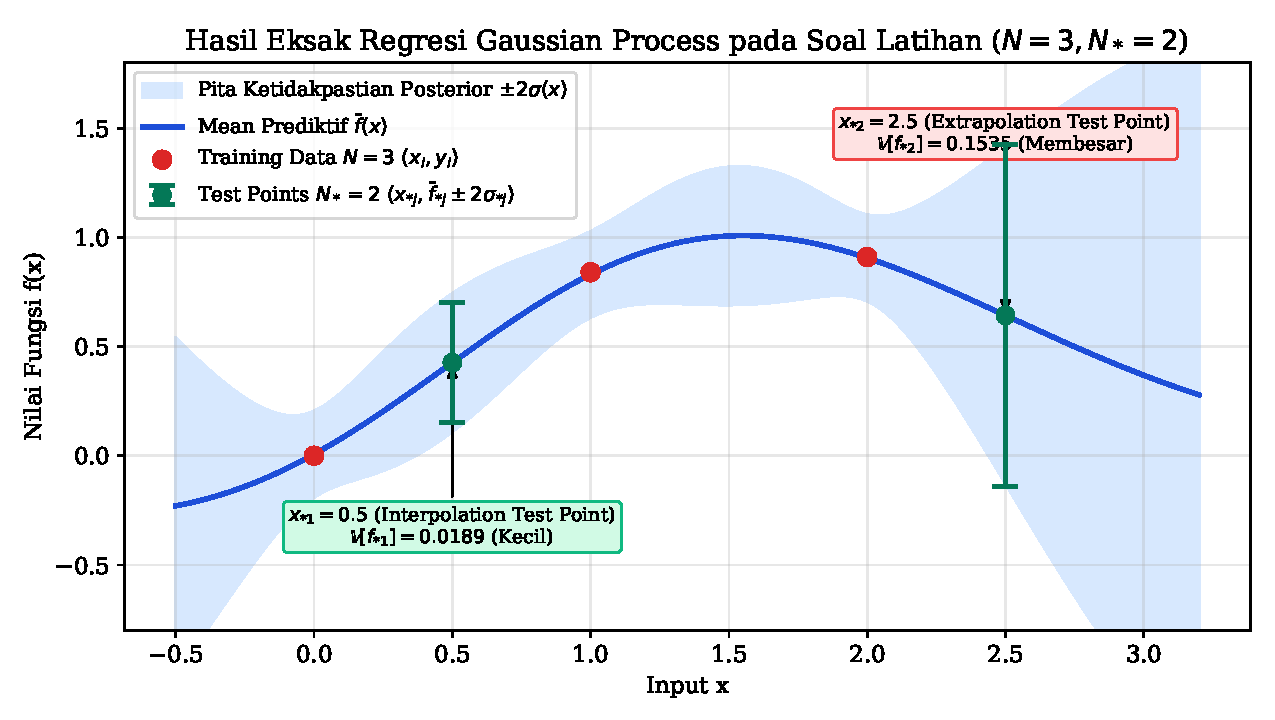
\includegraphics[width=0.9\textwidth]{fig5_worked_example.pdf}
\caption{Hasil Eksak Regresi Gaussian Process pada Soal Trainingan ($N=3, N_*=2$): Menampilkan kurva mean kontinu $\bar{f}(x)$, pita ketidakpastian posterior $95\%$ ($\pm 2\sigma(x)$), serta posisi kedua test point $x_{*1}=0.5$ dan $x_{*2}=2.5$.}
\label{fig:worked_example}
\end{figure}

Dari hasil matriks kovariansi posterior di atas, kita peroleh variansi individual dan deviasi standar untuk masing-masing test point:
\begin{itemize}
    \item \textbf{Titik Interpolasi ($x_{*1} = 0.5$)}:
    \begin{equation}
    \mathbb{V}[f_{*1}] = [\operatorname{cov}(\mathbf{f}_*)]_{11} = \mathbf{0.0251} \implies \sigma_{*1} = \sqrt{0.0251} \approx \mathbf{0.1584}
    \end{equation}
    Karena $x_{*1} = 0.5$ diapit sangat dekat oleh data observasi $x_1 = 0.0$ dan $x_2 = 1.0$, data memberikan reduksi ketidakpastian yang masif, menyusutkan variansi dari prior $1.0000$ menjadi hanya $0.0251$ (terjadi reduksi ketidakpastian sebesar $97.5\%$).
    \item \textbf{Titik Ekstrapolasi ($x_{*2} = 2.5$)}:
    \begin{equation}
    \mathbb{V}[f_{*2}] = [\operatorname{cov}(\mathbf{f}_*)]_{22} = \mathbf{0.1483} \implies \sigma_{*2} = \sqrt{0.1483} \approx \mathbf{0.3851}
    \end{equation}
    Titik $x_{*2} = 2.5$ berada di luar rentang observasi training samples (data terjauh berada di $x_3 = 2.0$). Oleh karena itu, variansinya hampir $6\times$ lipat lebih besar dibanding titik interpolasi, secara matematis membuktikan bahwa model mengekspresikan ketidakpastian epistemik yang tinggi di area tanpa observasi.
    \item \textbf{Korelasi Silang Posterior}: Elemen non-diagonal bernilai positif ($[\operatorname{cov}(\mathbf{f}_*)]_{12} = 0.0241 > 0$), menunjukkan bahwa meskipun kedua test point terpisah sejauh $\Delta x = 2.0$, keduanya tetap mempertahankan kovariansi positif yang lemah sesuai kontinuitas fungsi kernel.
\end{itemize}

% =========================================================================
% BAGIAN 9: KESIMPULAN & PENUTUP
% =========================================================================
\section{Kesimpulan \& Relevansi terhadap Tugas Akhir}
\label{sec:kesimpulan}

Dokumen kredit ini telah membuktikan secara tuntas dan presisi seluruh fondasi matematis dari \textit{Gaussian Process Regression}:
\begin{enumerate}
    \item Penurunan analitik distribusi posterior bersyarat via partisi matriks Schur Complement telah dijabarkan lengkap dengan dimensi setiap variabel aljabar liniernya.
    \item Prinsip seleksi model otomatis (Occam's razor) melalui dekomposisi log marginal likelihood telah diuraikan dekonstruksi matematisnya.
    \item Komputasi stabil menggunakan algoritma Cholesky dua tahap (forward dan backward substitution) telah didemonstrasikan perhitungannya angka per angka pada contoh soal $N = 3, N_* = 2$.
    \item \textbf{Jembatan Teoretis ke Tugas Akhir}: Analisis komputasi pada Bagian~\ref{sec:cholesky} memperlihatkan bahwa inversi matriks membutuhkan waktu $\mathcal{O}(N^3)$ dan memori $\mathcal{O}(N^2)$. Apabila GP diterapkan langsung pada tugas \textit{Image Segmentation} di mana setiap piksel citra ($H \times W \times C$) menjadi satu data titik ($N > 10^5$), model GP standar tidak akan mampu dieksekusi secara komputasi. Temuan teoretis ini menjadi justifikasi fundamental mengapa pada sesi berikutnya kita mutlak membutuhkan metode \textit{Sparse Gaussian Process} (Inducing Points) dan \textit{Deep Gaussian Process} (DGP).
\end{enumerate}

\vspace{0.8cm}
\noindent
\textbf{Lampiran / Berkas Terkait}:
\begin{itemize}
    \item Kode Sumber LaTeX: \texttt{04\_dokumen\_ta/kredit\_bimbingan\_02.tex}
    \item Aset Visualisasi: \texttt{04\_dokumen\_ta/figures/}
    \item Skrip Pembuat Grafik: \texttt{04\_dokumen\_ta/generate\_figures.py}
\end{itemize}

\end{document}
